
\documentclass[ucs]{beamer}

\usetheme{GSyC}
%\usebackgroundtemplate{\includegraphics[width=\paperwidth]{gsyc-bg.png}}


\usepackage[spanish]{babel}   
\usepackage[utf8x]{inputenc}
\usepackage{graphicx}
\usepackage{amssymb} % Simbolos matematicos
\usepackage{lmodern,textcomp}  % para usar el carácter € tal cual
%\usepackage{hthtml}
%\usepackage{html}



% Metadatos del PDF, por defecto en blanco, pdftitle no parece funcionar
   \hypersetup{%
     pdftitle={Bootstrap},
     %pdfsubject={Diseño y Administración de Sistemas y Redes},%
     pdfauthor={GSyC},%
     pdfkeywords={},%
   }
%


% Para colocar un logo en la esquina inferior de todas las transpas
%   \pgfdeclareimage[height=0.5cm]{gsyc-logo}{gsyc}
%   \logo{\pgfuseimage{gsyc-logo}}


% Para colocar antes de cada sección una página de recuerdo de índice
%\AtBeginSection[]{
%  \begin{frame}<beamer>{Contenidos}
%    \tableofcontents[currentframetitle]
%  \end{frame}
%}



\begin{document}

% Entre corchetes como argumento opcional un título o autor abreviado
% para los pies de transpa
\title[Bootstrap]{Bootstrap}
%\subtitle{Diseño y Administración de Sistemas y Redes}
\author[GSyC]{Escuela Técnica Superior de Ingeniería de Telecomunicación\\
Universidad Rey Juan Carlos}
\institute{gsyc-profes (arroba) gsyc.urjc.es}
\date[2017]{Octubre de 2017}


%% TÍTULO
\begin{frame}
  \titlepage
  % Oportunidad para poner otro logo si se usó la opción nologo
  % \includegraphics[width=2cm]{logoesp}  
\end{frame}



%% LICENCIA DE REDISTRIBUCIÓN DE LAS TRANSPAS
%% Nota: la opción b al frame le dice que justifique el texto
%% abajo (por defecto c: centrado)
\begin{frame}[b]



\vspace{1cm}
\begin{footnotesize}

\begin{flushright}
{


Derivado a partir de material de \\
Jesús M. González-Barahona y Gregorio Robles.

El original está disponible en \\
\url{http://cursosweb.github.io}\\
  Algunos derechos reservados. \\
  Este trabajo se distribuye bajo la licencia \\
  Creative Commons Attribution Share-Alike 4.0\\
}


\end{flushright}  


\end{footnotesize}
\end{frame}



%% ÍNDICE
%\begin{frame}
%  \frametitle{Contenidos}
%  \tableofcontents
%\end{frame}




% $Id$
%

\section{Bootstrap}
\subsection{Características}


%%---------------------------------------------------------------

\begin{frame}
\frametitle{¿Qué es Bootstrap?}

\begin{itemize}
  \item Bootstrap es un framework libre para desarrollo web
  \item Desarrollado inicialmente en 2011 por ingenieros de Twitter
  \item Incluye plantillas HTML y CSS con tipografías, formas, botones, cuadros, barras de navegación, carruseles de imágenes y muchas otras
  \item También existe la posibilidad de utilizar plugins de JavaScript
  \item Aunque su preferencia es \emph{mobile first}, permite crear diseños que se ven bien en múltiples dispositivos (\emph{responsive design})
\item
Orientado a programadores, no a diseñadores gráficos
\item
Es posiblemente la herramienta más popular para este fin, aunque hay alternativas
como Foundation


\end{itemize}

\end{frame}

%%---------------------------------------------------------------

\begin{frame}
\frametitle{Características de Bootstrap}

Ventajas 

\begin{itemize}
  \item Resulta sencillo y rápido escribir páginas con muy buen aspecto
  \item Se adapta a distintos dispositivos (\emph{responsive design})
  \item Proporciona un diseño consistente
  \item Es compatible con los navegadores modernos
  \item Es software libre
\end{itemize}

Inconvenientes

    \begin{itemize}
    \item
Al ser una herramienta muy popular, las páginas web que no 
estén personalizadas \emph{quedan iguales
que las de todo el mundo}

    \item
Alternativas como Foundation pueden resultar más convenientes
para personalizar los estilos
    \end{itemize}

\end{frame}

%%---------------------------------------------------------------

\begin{frame}[fragile]
\frametitle{Ficheros de Bootstrap}

\begin{footnotesize}
\begin{verbatim}
bootstrap/
|--- css/
|   |--- bootstrap.css
|   |--- bootstrap.css.map
|   |--- bootstrap.min.css
|   |--- bootstrap-theme.css
|   |--- bootstrap-theme.css.map
|   |--- bootstrap-theme.min.css
|--- js/
|   |--- bootstrap.js
|   |--- bootstrap.min.js
|--- fonts/
    |--- glyphicons-halflings-regular.eot
    |--- glyphicons-halflings-regular.svg
    |--- glyphicons-halflings-regular.ttf
    |--- glyphicons-halflings-regular.woff
    |--- glyphicons-halflings-regular.woff2
\end{verbatim}
\end{footnotesize}

\end{frame}


%%---------------------------------------------------------------

\begin{frame}[fragile]
\frametitle{Holamundo en Bootstrap}


%\begin{scriptsize}
%\begin{verbatim}
%<!DOCTYPE html>
%<html>
%<head>
%  <meta charset="utf-8">
%  <title>Basic Bootstrap Template</title>
%  <meta name="viewport" content="width=device-width, initial-scale=1.0">
%  <link rel="stylesheet" type="text/css" href="css/bootstrap.min.css">
%</head>
%<body>
%  <h1>Hello, world!</h1>
%  <script src="http://code.jquery.com/jquery.min.js"></script>
%  <script src="js/bootstrap.min.js"></script>
%</body>
%</html>
%\end{verbatim}
%\end{scriptsize}

  \begin{scriptsize}
  \begin{verbatim}
<!DOCTYPE html>
<html lang="es-ES">
<head>
  <meta charset="utf-8">
  <title>Hola mundo en bootstrap</title>
  <meta name="viewport" content="width=device-width, initial-scale=1.0">
  <link rel="stylesheet" 
     href="https://maxcdn.bootstrapcdn.com/bootstrap/3.3.7/css/bootstrap.min.css">
  <script 
     src="https://ajax.googleapis.com/ajax/libs/jquery/3.2.0/jquery.min.js">
  </script>
  <script 
     src="https://maxcdn.bootstrapcdn.com/bootstrap/3.3.7/js/bootstrap.min.js">
  </script>
</head>
<body>
  <div class="container">
    <h1>
      Hola, bootstrap
    </h1>
  </div>
</body>
</html>
  \end{verbatim}
  \end{scriptsize}
\end{frame}



%%---------------------------------------------------------------

\begin{frame}[fragile]
\frametitle{Bootstrap en CDN}

\begin{itemize}
  \item Con un CDN (Content Delivery Network) no hace falta tener Bootstrap en nuestros
archivos. Además, si un usuario ya ha descargado esas URLs, probablemente
las tenga ya en la caché del navegador (con el consiguiente ahorro de tiempo).
\end{itemize}

\begin{scriptsize}
\begin{verbatim}
 <!-- Latest compiled and minified CSS -->
<link rel="stylesheet" 
href="http://maxcdn.bootstrapcdn.com/bootstrap/3.3.7/css/bootstrap.min.css">

<!-- jQuery library -->
<script 
 src="https://ajax.googleapis.com/ajax/libs/jquery/1.11.1/jquery.min.js">
</script>

<!-- Latest compiled JavaScript -->
<script 
 src="http://maxcdn.bootstrapcdn.com/bootstrap/3.3.7/js/bootstrap.min.js">
</script>
\end{verbatim}
\end{scriptsize}
\end{frame}


%%---------------------------------------------------------------
\begin{frame}[fragile]
\frametitle{Viewport}
Para diseñar webs en dispositivos móviles, es importante tener
claro qué es el \emph{viewport} y cómo se comporta en este
tipo de dispositivos
\begin{itemize}
\item
\emph{Viewport} es la zona visible de una página web. En los navegadores
tradicionales de escritorio, coincide con la ventana del navegador

\item
Supongamos una página web grande y compleja, como la portada de un
periódico.
La página no cabrá en la ventana del navegador, el usuario usará
las barras de scroll para mover el
\emph{viewport} 
sobre el documento.

Al redimensionar la ventana, cambiará el tamaño del
\emph{viewport} 

\item

Cambiar el tamaño del viewport reposiciona el texto: las líneas se truncan
para adaptarse a ese tamaño.
\end{itemize}

\emph{Viewport} 
es un rectángulo donde se compone un fragmento (tal vez completo)
de la página web para presentarla al usuario
\end{frame}



%%---------------------------------------------------------------
\begin{frame}[fragile]
\frametitle{}
Con la aparición de los navegadores en teléfonos móviles, esto cambia
\begin{itemize}
\item
El área visible de un móvil es demasiado pequeña, componer una página web tradicional
en ese 
\emph{viewport} 
quedaría mal

\item
Además, en un navegador para móvil, no hay barras de scroll, ni ventanas
\end{itemize}


\end{frame}

%%----------------------------------------------
\begin{frame}[fragile]

Para solucionar este problema (en las páginas tradicionales),  se usa un 
\emph{viewport} virtual, mayor que el 
\emph{viewport} ordinario (la pantalla)



    \begin{itemize}
    \item
Lo introduce Apple para Safari en iOS, luego pasa a ser estándar

    \item
El ancho del 
\emph{viewport} 
virtual es razonablemente grande, por ejemplo 980
pixeles en el navegador safari para iPhone

    \item
El navegador compone la página sobre este viewport virtual, ya no hacen
falta barras desplazamiento horizontal

    \item
El usuario arrastra el 
\emph{viewport} 
(la pantalla, más pequeña) sobre el viewport virtual,
para que le muestre una zona u otra del documento. También se le puede permitir
hacer zoom
    \end{itemize}

\end{frame}




%%---------------------------------------------------------------
\begin{frame}[fragile]
\frametitle{Páginas responsive}

Una página web moderna con un minimo de calidad se entiende
que tiene que ser 
\emph{responsive}
\begin{itemize}
\item
La página se adapta al tamaño de la pantalla (escritorio, tablet, móvil),
sin necesidad de barras de desplazamiento horizontal

\item
El diseño 
\emph{responsive}
tal y como lo conocemos en la actualidad se basa
en el uso de un
\emph{grid}. En español se traduce por 
cuadrícula o rejilla

\item
En estas páginas ya no hace falta un
\emph{viewport} virtual, 
porque la página está diseñada para adaptarse al
\emph{viewport} 
ordinario (la pantalla pequeña)


\end{itemize}

\end{frame}




%%---------------------------------------------------------------
\begin{frame}[fragile]
\frametitle{}
La misma cuadrícula de 12 elementos se presenta de forma distinta
en un ordenador

  \begin{center}
  \begin{footnotesize}
XXX

XXX
  \end{footnotesize}
  \end{center}


En un tablet
  \begin{center}
  \begin{footnotesize}
XX

XX

XX
  \end{footnotesize}
  \end{center}


En un móvil
  \begin{center}
  \begin{footnotesize}
X

X

X

X

X

X
  \end{footnotesize}
  \end{center}
\end{frame}


%%---------------------------------------------------------------

\begin{frame}[fragile]
\frametitle{Responsive design}

\begin{center}
\begin{figure}[p]
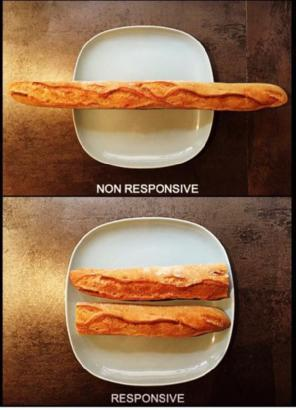
\includegraphics[width=0.47\textwidth]{figs/responsive.jpg}
\end{figure}
\end{center}

\begin{flushright}
{\tiny
Foto: https://image-store.slidesharecdn.com/420d15aa-cbf0-4ded-ac42-fcf728610bc1-original.jpeg
}
\end{flushright}

\end{frame}


%%---------------------------------------------------------------

\begin{frame}
\frametitle{Bootlint}

\begin{itemize}
  \item Herramienta que detecta algunos errores comunes el HTML de diseños \texttt{Bootstrap}
  \item Comprueba que las instancias de componentes Bootstrap han sido correctamente estructurados
  \item Analiza también la inclusión de ciertas etiquetas $<meta>$, la declaración DOCTYPE HTML5, etc.
  \item Supone que el HTML es correcto, así que deberíamos usar previamente alguna herramienta como el W3C validator o similar
  \item Página web: \url{https://github.com/twbs/bootlint}
\end{itemize}
\end{frame}


%%---------------------------------------------------------------
\begin{frame}[fragile]
\frametitle{}


\begin{itemize}
\item
Instalación:
  \begin{footnotesize}
  \begin{verbatim}
apt-get install nodejs-legacy
npm install -g bootlint
  \end{verbatim}
  \end{footnotesize}
\item
bootlint mostrará un warning

  \begin{footnotesize}
  \begin{verbatim}
missing X-UA-Compatible <meta> tag that disables 
old IE compatibility modes
  \end{verbatim}
  \end{footnotesize}


    \begin{itemize}
    \item
Internet Explorer 6 (años 2001-2008) fue un navegador muy usado, que no seguía
las normas HTML
    \item
Durante algún tiempo pudo ser recomendable que quien usase HTML estándar (y no HTML IE 6),
lo indicara con

  \begin{footnotesize}
  \begin{verbatim}
<meta http-equiv="X-UA-Compatible" content="IE=edge">
  \end{verbatim}
  \end{footnotesize}

    \item
En la actualidad, añadir esta indicación se considera obsoleto.
Podemos ignorar este warning de bootlint
    \end{itemize}
\end{itemize}

\end{frame}



%%---------------------------------------------------------------

\begin{frame}[fragile]
\frametitle{Mobile first}

% Info: https://developer.mozilla.org/es/docs/M%C3%B3vil/Viewport_meta_tag

\begin{itemize}
  \item Con una propiedad de etiqueta meta, podemos indicar la escala inicial del \emph{viewport}
 
\item
Como las páginas con bootstrap son
\emph{responsive}
es habitual especificar que el
\emph{viewport}
virtual coincida con el ancho de la pantalla, esto es, con el 
\emph{viewport}
ordinario

\end{itemize}

\begin{footnotesize}
\begin{verbatim}
<meta name="viewport" content="width=device-width, initial-scale=1">
\end{verbatim}
\end{footnotesize}

\begin{itemize}
  \item También se puede inhabilitar el zoom en dispositivos móviles con \texttt{user-scalable=no}
  \item Los usuarios sólo podrán hacer \emph{scroll} y tendrá una apariencia nativa.
  \item Usar con precaución. No vale para todas las aplicaciones
\end{itemize}

\begin{footnotesize}
\begin{verbatim}
<meta name="viewport" content="width=device-width, initial-scale=1, 
maximum-scale=1, user-scalable=no">
\end{verbatim}
\end{footnotesize}

\end{frame}


\subsection{Rejilla de Bootstrap}
%%---------------------------------------------------------------

\begin{frame}[fragile]
\frametitle{Contenedores}

\begin{itemize}
   \item Todos los elementos de Bootstrap deben estar dentro de un elemento contenedor
   \item Para un contenedor responsivo de tamaño fijo, se usa \texttt{.container}
\end{itemize}

\begin{footnotesize}
\begin{verbatim}
<div class="container">
  ...
</div>
\end{verbatim}
\end{footnotesize}

\begin{itemize}
  \item Si se desea un contenedor con el ancho total (del \emph{viewport}), se ha de usar \texttt{.container-fluid}
\end{itemize}

\begin{footnotesize}
\begin{verbatim}
<div class="container-fluid">
  ...
</div>
\end{verbatim}
\end{footnotesize}


    \begin{itemize}
    \item
Los contenedores no se pueden anidar
    \end{itemize}


\end{frame}



%%---------------------------------------------------------------

\begin{frame}
\frametitle{El sistema de rejilla (I)}

El diseño de páginas basado en rejilla se realiza mediante filas y
columnas donde se colocan los contenidos. Así funciona la rejilla de Bootstrap:

\begin{itemize}

  \item Filas, dentro un contenedor, agrupan horizontalmente varias columnas, que son las que tienen contenido
  \item La pantalla se divide en 12 columnas
  \item Las columnas definen su anchura especificando cuántas columnas de la fila ocupan
  \item Hay clases CSS (como por ejemplo .row y .col-xs-4) para crear rejillas rápidamente
  \item Hay padding entre columnas. En la primera y última columnas, las filas (elementos .row) aplican márgenes negativos

\end{itemize}

\end{frame}

%%---------------------------------------------------------------

\begin{frame}[fragile]
\frametitle{El sistema de rejilla (II)}

% Ejemplos: http://getbootstrap.com/examples/grid/

\begin{center}
\begin{figure}[p]
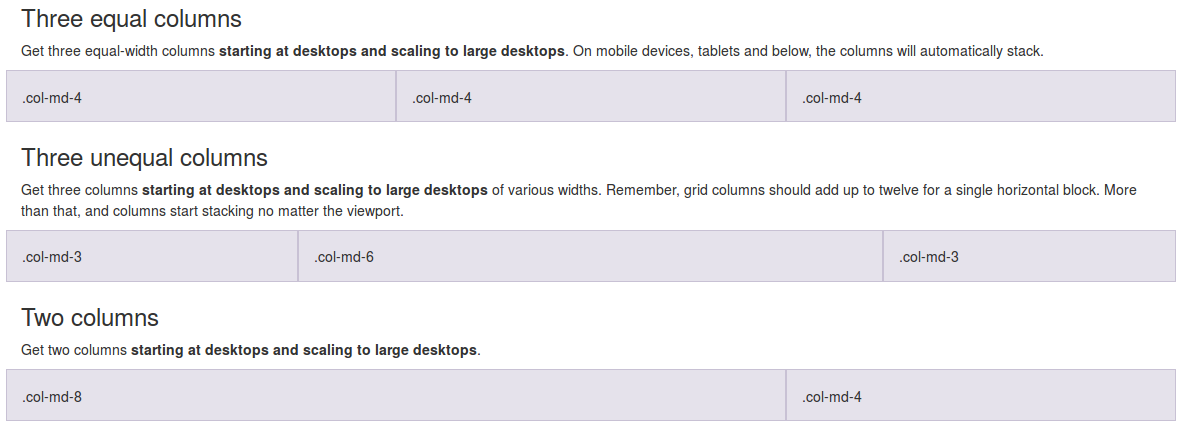
\includegraphics[width=0.99\textwidth]{figs/grid.png}
\end{figure}
\end{center}

\end{frame}







%%---------------------------------------------------------------

\begin{frame}[fragile]
\frametitle{Responsive design en Bootstrap}

Móviles y escritorio:

\begin{center}
\begin{figure}[p]
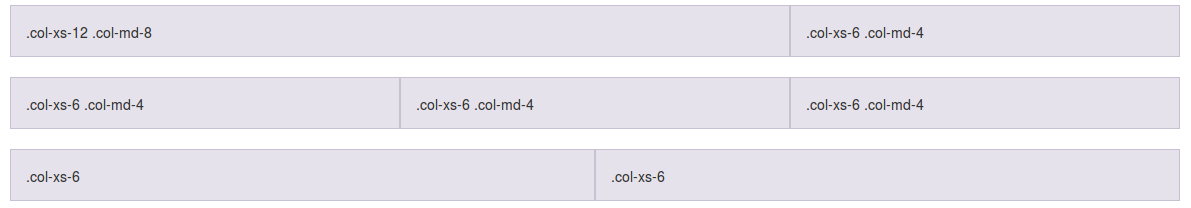
\includegraphics[width=0.99\textwidth]{figs/grid-responsive.png}
\end{figure}
\end{center}

Móvil, tableta y escritorio:

\begin{center}
\begin{figure}[p]
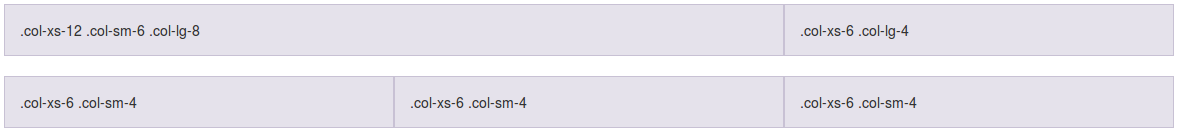
\includegraphics[width=0.99\textwidth]{figs/grid-responsive2.png}
\end{figure}
\end{center}

\end{frame}


%%---------------------------------------------------------------
\begin{frame}[fragile]
\frametitle{El sistema de rejilla (III)}
Dicho de otro modo

\begin{itemize}
\item
El ancho de cada columna se mide en casillas

\item
La pantalla ocupa un ancho total de 12 casillas, que repartimos
entre el número de columnas que deseemos

\item
Si el
\emph{viewport} 
(la pantalla) es lo bastante ancho, las columnas
se muestran en su disposición ordinaria, esto es, cada una al lado
de la otra

\item
Si el 
\emph{viewport} 
es demasido pequeño, entonces las casillas se apilan verticalmente

\end{itemize}
\end{frame}


%%---------------------------------------------------------------
\begin{frame}[fragile]
\frametitle{}


Hay 4 tipos de casillas, según el ancho del 
\emph{viewport} 
disponible en el dispositivo

\begin{itemize}
\item
lg

Large. Pantallas alta resolución.
1200 pixels y más

\item
md

Medium. 
Pantallas tradicionales.
992-1199 pixeles

\item
sm

Small. Tablets.
768-991 pixeles

\item
xs

Extra small. Teléfonos moviles.
767 pixeles o menos
\end{itemize}

La frontera entre cada uno de estos tamaños se denomina
\emph{breackpoint}
\end{frame}



%%---------------------------------------------------------------
\begin{frame}[fragile]
\frametitle{}
\begin{itemize}
\item
Columnas
\emph{lg}

Disposición normal en
pantallas 
grandes

se apilan en:
pantallas
medianas, pequeñas o muy pequeñas


\item
Columnas
\emph{md}

Disposición normal en
pantallas medianas o grandes

Se apilan en pantallas pequeñas o muy pequeñas


\item
Columnas
\emph{sm}

Disposición normal en 
pantallas pequeñas, medianas o grandes

Se apilan en
pantallas muy pequeñas


\item
Columnas
\emph{xs}

Disposición normal en 
pantallas muy pequeñas, medianas o grandes.

Nunca se apilan

\end{itemize}

\end{frame}



%%---------------------------------------------------------------
\begin{frame}[fragile]
\frametitle{}
Dicho de otro modo
\begin{itemize}
\item
Cada tipo de columna se muestra en su disposición normal,
esto es, horizontalmente, si la pantalla es de su 
tipo o de un tipo mejor

\item
En otro caso, las casillas se apilan verticalmente
\end{itemize}

Esto parece un poco complicado, pero con el siguiente ejemplo
verás que no:

    \begin{enumerate}
    \item
Vete a 

\url{http://ortuno.es/grid}

    \item
Maximiza la ventana

    \item
Vete reduciéndola gradualmente

    \end{enumerate}

\end{frame}



%%---------------------------------------------------------------
\begin{frame}[fragile]
\frametitle{Columnas desplazadas}
Además de indicar el ancho de una columna, podemos especificar
que se desplace un cierto número de casillas a la derecha, esto es, que se dejen casillas en blanco 


Basta añadir un nuevo valor al atributo class del div
\begin{itemize}
\item
\verb|col-lg-offset-N|

\item
\verb|col-md-offset-N|

\item
\verb|col-sm-offset-N|

\item
\verb|col-xs-offset-N|

\end{itemize}

Donde N es el número de casillas, entre 1 y 11

Ejemplo

\verb|<div class="col-md-4 col-md-offset-4">|
\end{frame}



%%---------------------------------------------------------------

%\begin{frame}[fragile]
%\frametitle{Media queries}

%Bootstrap utiliza \emph{media queries} para establecer puntos de ruptura en los que la rejilla se transforma para adaptarse a cada dispositivo.
%
%\begin{footnotesize}
%\begin{verbatim}
%/* Extra small devices (phones, less than 768px) */
%/* No media query since this is the default in Bootstrap */
%
%/* Small devices (tablets, 768px and up) */
%@media (min-width: @screen-sm-min) { ... }
%/* Medium devices (desktops, 992px and up) */
%@media (min-width: @screen-md-min) { ... }
%/* Large devices (large desktops, 1200px and up) */
%@media (min-width: @screen-lg-min) { ... }
%\end{verbatim}
%\end{footnotesize}
%
%
%Se pueden utilizar también \emph{media queries} que definen la propiedad max-width y restringen los dispositivos a los que se aplican los estilos:
%
%\begin{footnotesize}
%\begin{verbatim}
%@media (max-width: @screen-xs-max) { ... }
%@media (min-width: @screen-sm-min) and (max-width: @screen-sm-max) { ... }
%@media (min-width: @screen-md-min) and (max-width: @screen-md-max) { ... }
%@media (min-width: @screen-lg-min) { ... }
%\end{verbatim}
%\end{footnotesize}
%
%
%\end{frame}


\subsection{Componentes de Bootstrap}
%%---------------------------------------------------------------

\begin{frame}
\frametitle{Componentes de Boostrap}

Bootstrap viene con una serie de estilos (generalmente en formato de clase CSS)
y componentes en JavaScript.

\begin{itemize}
  \item \texttt{panel}
  \item \texttt{btn}
  \item \texttt{nav}
  \item \texttt{dropdown}
  \item \texttt{carousel} 
  \item y otras utilidades responsivas
\end{itemize}

\end{frame}

%%---------------------------------------------------------------
\begin{frame}[fragile]
\frametitle{panel}
Un panel es un componente de bootstrap consistente en una caja redondeada donde se pueden
insertar
otros elementos 

\begin{itemize}
\item
Sintácticamente, es un div cuyo atributo class tiene el valor
\verb|panel|
y el valor del tipo de panel, que puede ser


    \begin{itemize}
    \item
\verb|panel-default|
    \item
\verb|panel-primary|
    \item
\verb|panel-success|
    \item
\verb|panel-info|
    \item
\verb|panel-warning|
    \item
\verb|panel-danger|
    \end{itemize}

\item
Cada panel se compone de

    \begin{itemize}
    \item
Cabecera: un div de clase
\verb|panel-heading|

    \item
Cuerpo: un div de clase
\verb|panel-body|
    \item
Pié: un div de clase
\verb|panel-footer|
    \end{itemize}

\end{itemize}

Ejemplo:

\url{http://ortuno.es/panel}

\end{frame}

%%---------------------------------------------------------------
\begin{frame}[fragile]
\frametitle{btn}

A partir de los elementos HTML
\verb|<a>|,
\verb|<button>| o
\verb|<input>|,
se puede generar un botón de Bootstrap, basta añadir la clase btn


    \begin{itemize}
    \item
Adicionalmente, se puede especificar el tipo de botón:
        btn-default
        btn-xs
        btn-sm
        btn-lg
        btn-block
        btn-primary
        btn-success
        btn-info
        btn-warning
        btn-link

    \end{itemize}
Ejemplo:

\url{http://ortuno.es/button}

\end{frame}





%%---------------------------------------------------------------
\begin{frame}[fragile]
\frametitle{nav}

\verb|nav| es un componente de Bootstrat formado por un conjunto de enlaces
para navegar dentro de un web. Hay tres tipos


    \begin{itemize}
    \item
\verb|nav-stacked|

Tipo por omisión. Enlaces apilados verticalmente
    \item
\verb|nav-tabs|

Enlaces en forma de pestaña

    \item
\verb|nav-pills|

Enlaces en forma de botón, llamados \emph{pills}
    \end{itemize}



\end{frame}

%%----------------------------------------------
\begin{frame}[fragile]


Sintácticamente, un 
\verb|nav| 
es 
    \begin{itemize}
    \item
Un elemento
\verb|<ul>| 
al que se añade el atributo
\verb|class| 
con el valor
\verb|nav| 
más el valor del tipo de nav:

\verb|nav-stacked|,
\verb|nav-tabs|,
\verb|nav-pills|

    \item
Cada uno de los enlaces es un
\verb|<li>| 
que contiene el 
\verb|<a>| 
correspondiente

    \item
Cada 
\verb|<li>| 
puede incluir, adicionalmente, el atributo
\verb|class| 
con el valor

    \begin{itemize}
    \item
\verb|active| 
para indicar que se trata del botón/pestaña actual

    \item
\verb|disabled| 
    \end{itemize}

    \end{itemize}


Ejemplo:

\url{http://ortuno.es/nav}

\end{frame}



%%---------------------------------------------------------------
\begin{frame}[fragile]
\frametitle{dropdown}
Un 
\verb|dropdown|
es un menú desplegable: un menú que aparece al pulsar 
\emph{algo}, llamado \emph{toggle}


    \begin{itemize}
    \item
El 
\verb|toggle|
puede ser
\begin{itemize}
\item
\verb|<a>|
\item
\verb|<btn>|, aislado o dentro de
\verb|<btn-group>|
\item
Una pestaña o un botón de un
\verb|nav|
ya sea
\verb|nav-stacked, nav-tabs|
o
\verb|nav-pills|
\item
Algunos otros elementos
\end{itemize}

    \item
El menú es un 
\verb|<ul>| con sus 
\verb|<li>| 

    \end{itemize}
El 
\verb|toggle|
y el 
\verb|<ul>| 
tienen que estar contenidos dentro de un elemento

    \begin{itemize}
    \item
Que tendrá la clase
\verb|<dropdown>| 
    \item
Podrá ser un 
\verb|div|
genérico
o un 
\verb|btn-group|, 
o un 
\verb|nav| 
    \end{itemize}

\end{frame}



%%---------------------------------------------------------------
\begin{frame}[fragile]
\frametitle{}
\begin{itemize}
\item
El toggle tiene que tener los atributos

  \begin{scriptsize}
  \begin{verbatim}
data-toggle="dropdown" class="dropdown-toggle"
  \end{verbatim}
  \end{scriptsize}


\item
Para que el usuario sepa que el toggle es desplegable, se
añade el símbolo \emph{caret}, también llamado acento
circunflejo (un pequeño triángulo apuntando hacia abajo) 

  \begin{scriptsize}
  \begin{verbatim}
<span class="caret"></span>
  \end{verbatim}
  \end{scriptsize}

% En realidad es un caret invertido. El caret se usa tradicionalmente en las
% revisiones del texto de imprenta, para indicar que falta un símbolo (una coma,
% un punto) Viene del latín carare, "falta"



\item
El
\verb|<ul>|
del menú tendrá los atributos

  \begin{scriptsize}
  \begin{verbatim}
<ul class="dropdown-menu">
  \end{verbatim}
  \end{scriptsize}


\end{itemize}

Ejemplo:

\url{http://ortuno.es/dropdown}
\end{frame}



\subsection{formularios}
%%---------------------------------------------------------------
\begin{frame}[fragile]
\frametitle{Formularios}
Bootstrap incluye clases para mejorar el aspecto y usabilidad de los
formularios
\begin{itemize}
\item
El uso de 
\verb|<label>|
es necesario, no es válido escribir texto HTML para identificar los
elementos del formulario

\item
Cada par 
\verb|<label>| 
- elemento de entrada (\verb|<select>|,
\verb|<textarea>|, etc)
label tiene que ir dentro de un
\verb|<div>|
de clase 
\verb|form-group|

\item
Los elementos de entrada de texto tienen que llevar la clase 
\verb|form-control|
(los checkbox, radiobutton y similares, no)
\end{itemize}
Esto hace, entre otras cosas, que los elementos de entrada ocupen
todo el ancho del container
\end{frame}


%%---------------------------------------------------------------
\begin{frame}[fragile]
\frametitle{}

  \begin{scriptsize}
  \begin{verbatim}
    <form action="/action_page.html">

      <div class="form-group">
        <label for="usuario"> Nombre de usuario:</label>
        <input type="text" id="usuario" class="form-control" name="usuario">
      </div>

      <div class="form-group">
        <label for="contrasenya"> Contraseña:</label>
        <input type="password" name="contrasenya" id="contrasenya" class="form-control">
      </div>

      <input type="submit">
    </form>
  \end{verbatim}
  \end{scriptsize}

\end{frame}



%%---------------------------------------------------------------
\begin{frame}[fragile]
\frametitle{Formulario inline}
La clase
\verb|form-inline|
ofrece una presentación más compacta del formulario, con
los campos en horizontal
\begin{itemize}
\item
Basta añadir 
\verb|class="form-inline"|
al elemento
\verb|<form>|
\end{itemize}


  \begin{scriptsize}
  \begin{verbatim}
    <form action="/action_page.html" class="form-inline">
       ...
    </form>
  \end{verbatim}
  \end{scriptsize}

Ejemplo con diversos formularios Bootstrap:

\url{http://ortuno.es/bform}

\end{frame}




%%---------------------------------------------------------------
\begin{frame}[fragile]
\frametitle{carousel}
El componente 
\verb|carousel| muestra fotografías como un pase de diapositivas, 
desplazándose horizontalmente y con un texto en cada una de ella

Un carousel es un div con los siguientes atributos


    \begin{itemize}
    \item
Clase \verb|carousel slide|

   \item
Atributo 
\verb|data-ride| 
con el valor
\verb|carousel| 
para especificar que el carrusel se ponga en marcha en cuanto
se cargue la página

    \begin{itemize}
    \item
Si lo omitimos, el carrusel solo se mueve al hacer clic sobre controles izquierda y derecha
    \end{itemize}



   \item
Atributo
\verb|id| con el 
identificador
de carousel

   \item
La velocidad de transición de las diapositivas se puede especificar, en milisegundos,
con el atributo
\verb|data-interval|

Su valor por omisión es 5000
    \end{itemize}




\end{frame}

%%----------------------------------------------
\begin{frame}[fragile]
Dentro del 
\verb|div|
principal de carousel habrá:

\begin{itemize}
\item
Indicators

Son los círculos que aparecen debajo del texto para representar
la diapositiva activa respecto a todas las demás
\item
Un 
\verb|<div>|
de clase
\verb|<carousel-inner>|
con las fotos y el texto

\item
Controles izquierda y derecha
\end{itemize}


\end{frame}

%%----------------------------------------------
\begin{frame}[fragile]

Los indicators son una
\verb|<ol>|
de clase
\verb|carousel-indicators|

    \begin{itemize}
    \item
Cada
\verb|<li>|
del 
\verb|<ol>|
contiene un atributo
\verb|data-target|
con el identificador del carrusel 
y un 
\verb|data-slide-to|
con el ordinal de la imagen
    \end{itemize}

  \begin{scriptsize}
  \begin{verbatim}
 <ol class="carousel-indicators">
   <li data-target="#carrusel01" data-slide-to="0" class="active"></li>
   <li data-target="#carrusel01" data-slide-to="1"></li>
   <li data-target="#carrusel01" data-slide-to="2"></li>
 </ol>
  \end{verbatim}
  \end{scriptsize}


\end{frame}



%%---------------------------------------------------------------
\begin{frame}[fragile]
\frametitle{}
Cada diapositiva es un 
\verb|div|
de clase
\verb|item|

Contiene:
\begin{itemize}
\item
Un elemento
\verb|img|
con la imagen

\item
Un 
\verb|div|
de clase
\verb|carousel-caption|
con los textos
\end{itemize}

  \begin{scriptsize}
  \begin{verbatim}
<div class="item">
   <img src="images/foto02.jpg" alt="Segunda foto">
   <div class="carousel-caption">
      <h3>Título de la foto 2</h3>
      <p>Lorem Ipsum</p>
   </div>
</div>
  \end{verbatim}
  \end{scriptsize}

Una forma conveniente de redimensionar las fotos es especificar el atributo
\verb|width| directamente en cada imagen, dejando que el navegador fije el
alto manteniendo las proporciones

\end{frame}



%%---------------------------------------------------------------
\begin{frame}[fragile]
\frametitle{}
Los controles izquierda y derecha son elementos
\verb|<a>|

\begin{itemize}
\item
Contienen en el atributo 
\verb|href|
el identificador del carousel

\item
En el resto de atributos se indica qué caracter usar para el control

  \begin{scriptsize}
  \begin{verbatim}
<a class="left carousel-control" href="#carrusel01" data-slide="prev">
  <span class="glyphicon glyphicon-chevron-left"></span>
  <span class="sr-only">Previous</span>
</a>
<a class="right carousel-control" href="#carrusel01" data-slide="next">
  <span class="glyphicon glyphicon-chevron-right"></span>
  <span class="sr-only">Next</span>
</a>
  \end{verbatim}
  \end{scriptsize}
\end{itemize}

Ejemplo:

\url{http://ortuno.es/carousel}
\end{frame}



%%---------------------------------------------------------------

%\begin{frame}
%\frametitle{JavaScript}
%
%Con Bootstrap vienen una serie de \emph{plug-ins} de JavaScript, como:
%
%\begin{itemize}
%  \item transitions.js: efectos de transición
%  \item modal.js: diálogos simples y flexibles
%  \item dropdown.js: menús desplegables
%  \item scrollspy.js: según vamos bajando en la página, actualiza la \emph{navbar}
%  \item tab.js: pestañas
%  \item tooltip.js y popover.js: cajas con consejos o más información
%  \item alert.js: alertas
%  \item button.js: botones
%  \item collapse.js: permite mostrar/ocultar elementos
%  \item carousel.js: el (ya famoso carrusel)
%  \item affix.js: Menú de navegación lateral
%\end{itemize}
%
%\end{frame}




%%---------------------------------------------------------------

\begin{frame}
\frametitle{Enlaces relacionados}


\begin{itemize}
\item



S.F.Rahman. Jump Start Bootstrap. Ed SitePoint, 2014

\begin{tiny}
\url{http://proquest.safaribooksonline.com/book/web-design-and-development/9781457174346}
\end{tiny}

  \item Listado de recursos sobre Bootstrap \\
        \url{http://bootsnipp.com/resources}
  \item Bootsnipp: Cientos de componentes adicionales \\
        \url{http://www.bootsnipp.com}
  \item Startboostrap: Plantillas y temas Bootstrap (gratis) \\
        \url{http://startbootstrap.com/}  
  \item WrapBoostrap: Plantillas y temas Bootstrap (de pago) \\
        \url{https://wrapbootstrap.com/}
  \item BootTheme: Generador (no libre) de diseños Bootstrap \\
        \url{http://www.boottheme.com/}
\end{itemize}

\end{frame}



\end{document}

